\section{Problemstellung und Requirements}
\label{sec-3}
\begin{center}
	\fbox{
		\parbox{0.9\linewidth}{
			\textit{Ziel des Kapitels:}\\
			Anforderungen von technischer und anwendungsorientierter Seite darstellen und Problem formulieren.
	}}\\
\end{center}
%TODO formulierungen überarbeiten
Ziel dieser Arbeit ist am konkreten Beispiel der Helmholtz-Spule zu untersuchen, wie die HoloLens in der Physik Lehre eingesetzt werden kann. Dazu betrachtet die Arbeit speziell, wie der zuvor beschriebene Versuchsaufbau mit Informationen angereichert werden kann. Aufbauend auf den im vorigen Kapiteln erarbeiteten Hintergründen formulieren die folgenden Abschnitte an die Anwendung zu stellende Anforderungen aus anwendungsorientierter sowie technischer Sicht.\\

Wie kann die HoloLens für diesen Versuch konkret eingesetzt werden?\\

\begin{figure}[h!]
	\centering
	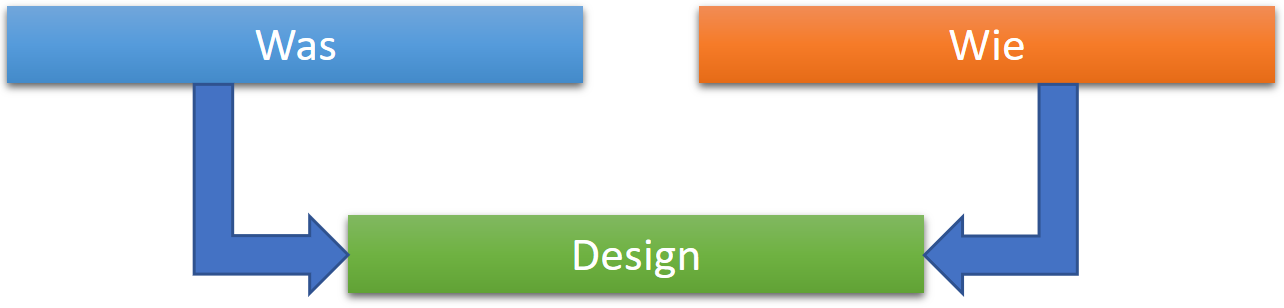
\includegraphics[width=0.6\textwidth]{images/Informiertes_Design.png}
	\caption{Informiertes Design}
	\label{img:Informiertes_Design}
\end{figure}

\subsection{Anforderungen}
\label{sec-3-1}
%TODO formulierungen überarbeiten
Die Anforderungen an eine Umsetzung kommen aus zwei Bereichen: Zum einen aus der Physik und zum anderen aus den technischen Modalitäten der HoloLens. Ein Design muss beide berücksichtigen und zusammenführen zu einer Lösung. Dabei bestimmt das Anwendungsszenario vor allem die inhaltlichen Anforderungen während die technischen Gegebenheiten eher auf das ''Wie'' der Umsetzung Einfluss nehmen. Zunächst sollen die inhaltlichen Anforderungen aufgestellt werden.

\subsubsection{Was - Physik}
Bla bla bla

\textit{Darzustellende Informationen:}
\begin{enumerate}
	\setlength{\itemsep}{-5pt}
	\item Magnetfeld von Erde und Spule
	\begin{itemize}[topsep=-0.25em]
		\setlength{\itemsep}{-0.25em}
		\item Stärke
		\item Richtung
		\item Homogenität
		\item Inhomogenität am Rand der Spule andeuten (Optional) 
	\end{itemize}
	\item Stromfluss durch die Spule
	\begin{itemize}[topsep=-0.25em]
		\setlength{\itemsep}{-0.25em}
		\item Richtung
		\item Kennzeichnung von Plus und Minus
		\item Stärke (Optional) 
	\end{itemize}
	\item Kompass
	\begin{itemize}[topsep=-0.25em]
		\setlength{\itemsep}{-0.25em}
		\item Nordrichtung
		\item Grobe Auslenkung der Nadel
	\end{itemize}
	\item Weitere Informationen (Optional)
	\begin{itemize}[topsep=-0.25em]
		\setlength{\itemsep}{-0.25em}
		\item Windungszahl der Spule
		\item Durchmesser und Abstand der Spulen
		\item Numerische Werte und Informationen (z.B. Fließt aktuell Strom, angelegte Stromstärke, angenommene Stärke des Erdmagnetfeldes, systematischer und zufälliger Fehler, etc.)
	\end{itemize}
\end{enumerate}

\textit{Nicht-funktionale Anforderungen:}
\begin{itemize}
	\setlength{\itemsep}{-5pt}
	\item Darstellungen müssen physikalisch korrekt und interpretierbar sein
	\item Nutzer darf nicht in seiner Interaktion mit dem Versuchsaufbau und relevanten Materialien eingeschränkt werden
	\item Anwendung soll benutzerfreundlich gestaltet sein
	\item Dazu sollen bestehende Empfehlungen und Hinweise zur Verbesserung der Nutzererfahrung einbezogen werden
\end{itemize}

\subsubsection{Wie - Technische Seite}
Technische Randbedingungen durch die Brille im Zusammenhang mit Anwendungsfall
\begin{itemize}
	\setlength{\itemsep}{-5pt}
	\item Größe, Geschwindigkeit, Farbe, Distanz zur Kamera von Objekten
	\item Zusammenspiel der Darstellungen mit der Umgebung beachten
	\item Stabilität der Hologramme gewährleisten
	\item 60 FPS stabil halten, stark spiegelnde oder transparente Oberflächen vermeiden, mögliche Einflüsse auf die Sensoren beachten
	\item Usability und UX Empfehlungen beachten
\end{itemize}

\subsection{Problemstellung}
\label{sec-3-2}
Zwei Aspekte: Anforderungen von der physikalischen und der technischen Seite

Problem: Anforderungen und technische Möglichkeiten sowie Einschränkungen zusammenbringen und eine Lösung entwickeln
\begin{itemize}
	\item Was soll dargestellt werden? (Was soll nicht dargestellt werden?)
	\item Wie soll es dargestellt werden?
	\item Wie soll damit interagiert werden?
\end{itemize}

